\appendix

\section{Few-shot regression collections}
\label{app:collections}

There is a dire need in the meta-learning community for standardised benchmarks, especially in the case of few-shot regression. To wit, meta-learning research is dominated by image classification, owing in part to the fact that such problems validate the assumptions of the field quite well -- learning to recognise shapes can indeed be learned accross a variety of classification tasks.

Thus, in the case of image classification, benchmarks exist. For instance, \citeauthor{triantafillou2019metadataset} from Google Research have proposed in \citeyear{triantafillou2019metadataset} ``Meta-Dataset'', a collection of image classification datasets to be used as a testbed by the community.

On the contrary, the few-shot regression community mostly relies on \textit{ad hoc} meta-datasets, with little systematic benchmarking other than on synthetic data. I for one believe that synthetic testing is most important in fundamental research, since it helps pinpoint the capabilities of an algorithm by controlling explicitly the assumptions one can make on the data. However, we do need to challenge ourselves to real-world applications, lest meta-learning remain a niche and unapplicable discipline.

In what follows, I describe four meta-datasets we work with at InVivo AI.

\subsection{A synthetic meta-dataset : the \texttt{Sinusoids} collection}
\label{app:collections-synthetic}

This synthetic few-shot regression benchmark, introduced by \citet{kim2018bayesian}, consists of 5,000 tasks defined by functions of the form :
\begin{align}
  y &= A \sin(\omega x + b) + \varepsilon &
  &\text{with}&
  &
  \begin{matrix}
    A \in \LB 0.1, 5.0 \RB \\
    b \in \LB 0.0, 2\pi \RB \\
    w \in \LB 0.5, 2.0 \RB \\
    \varepsilon \sim \normal \LP 0,(0.01 A)^2 \RP
  \end{matrix}&
\end{align}

The examples are generated by sampling inputs $x$ from the $[-5.0, 5.0]$ interval, as well as the observation noise $\varepsilon$. The tasks themselves are divided into a meta-train, a meta-validation and a meta-test sets, which contain respectively 56.25\%, 18.75\% and 25\% of the functions.

By design, this synthetic collection validates the assumptions of meta-learning : the functions are indeed sampled from a task distribution, and the goal of the algorithm is to learn to recognise the parameters of the sine function from very few points.

The \texttt{Sinusoids} collection, although it may be given other names, has become a standard benchmarking tool in the community.



\subsection{\texttt{Binding} and \texttt{Antibacterial}, two real-world collections}
\label{app:collections-real}

One important flaw in the \texttt{Sinusoids} collection is its lack of realism. Moreover as a drug discrovery company, InVivo AI strive to develop algorithms that work on real-world, bio-chemical data.

To that end we propose two collections, whose content is \href{https://github.com/invivoai/molecular-datasets}{available here}, compiled from data in the public domain. Both contain data from bioassays that are representative of real-world few-shot regression tasks that arise in drug discovery.

\begin{figure}[ht]
  \makebox[\linewidth][c]{
    \begin{subfigure}[t]{.5\textwidth}
      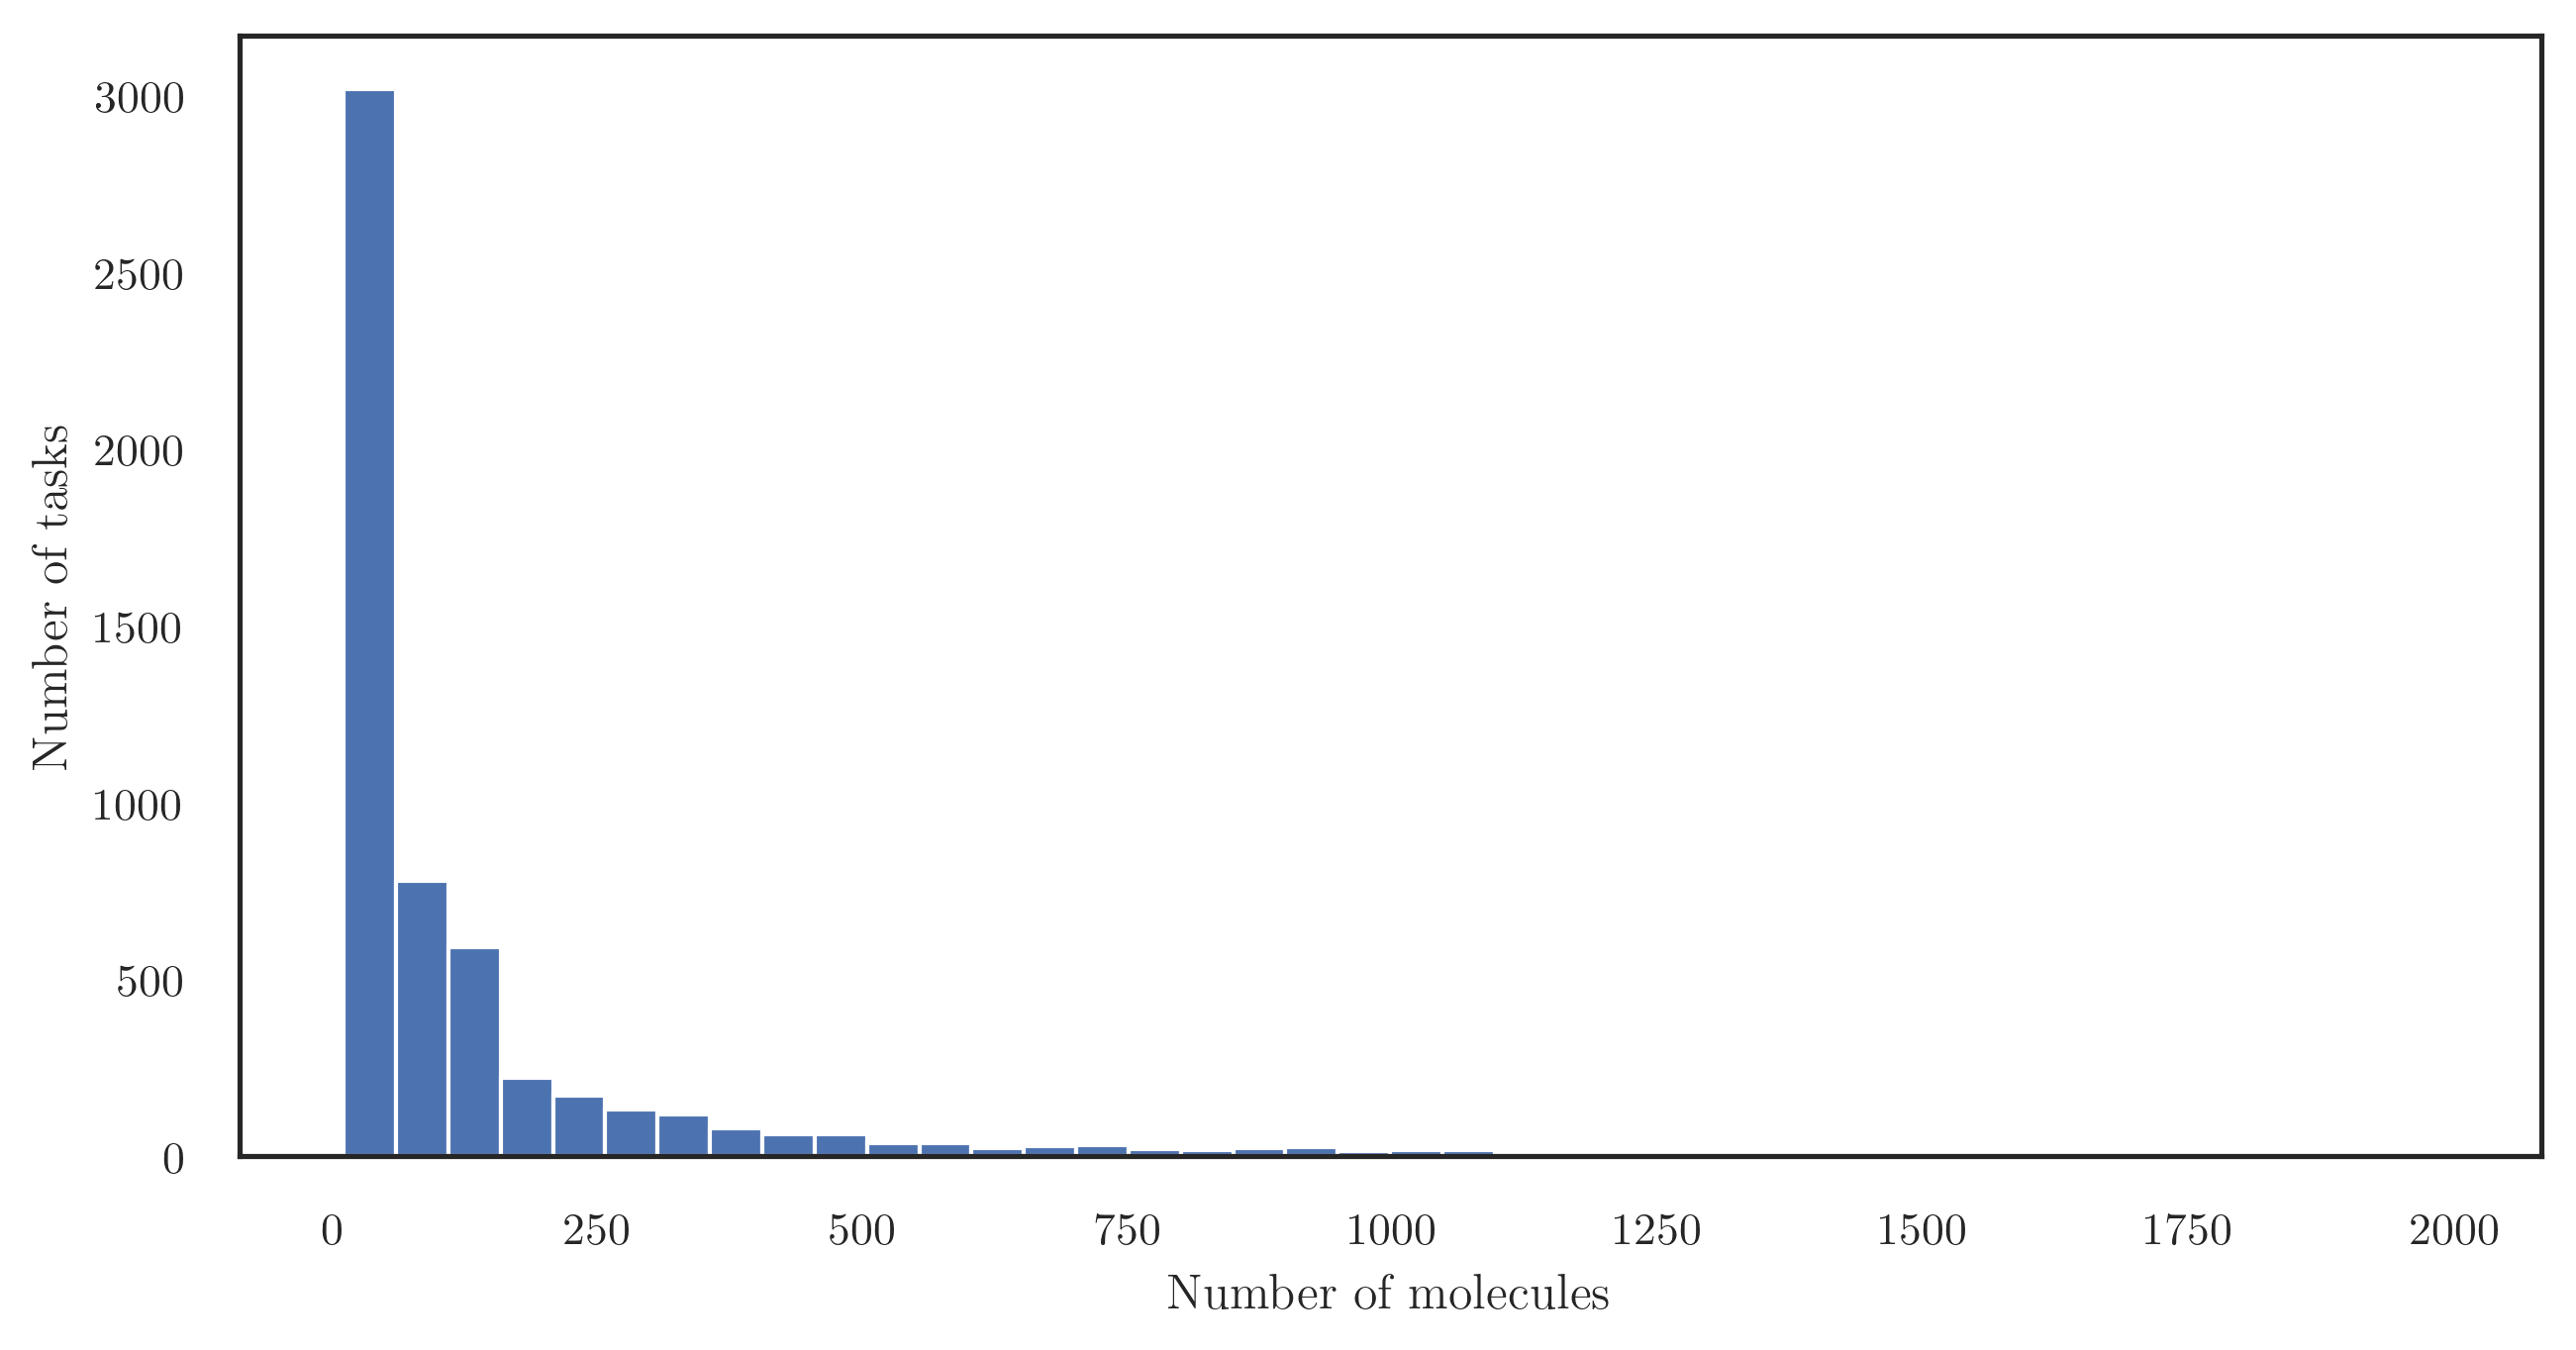
\includegraphics[width=1\textwidth,center]{datasets/hist-binding}
      \caption{\texttt{Binding}}
      \label{fig:hist-binding}
    \end{subfigure}
    \hspace{1cm}
    \begin{subfigure}[t]{.5\textwidth}
      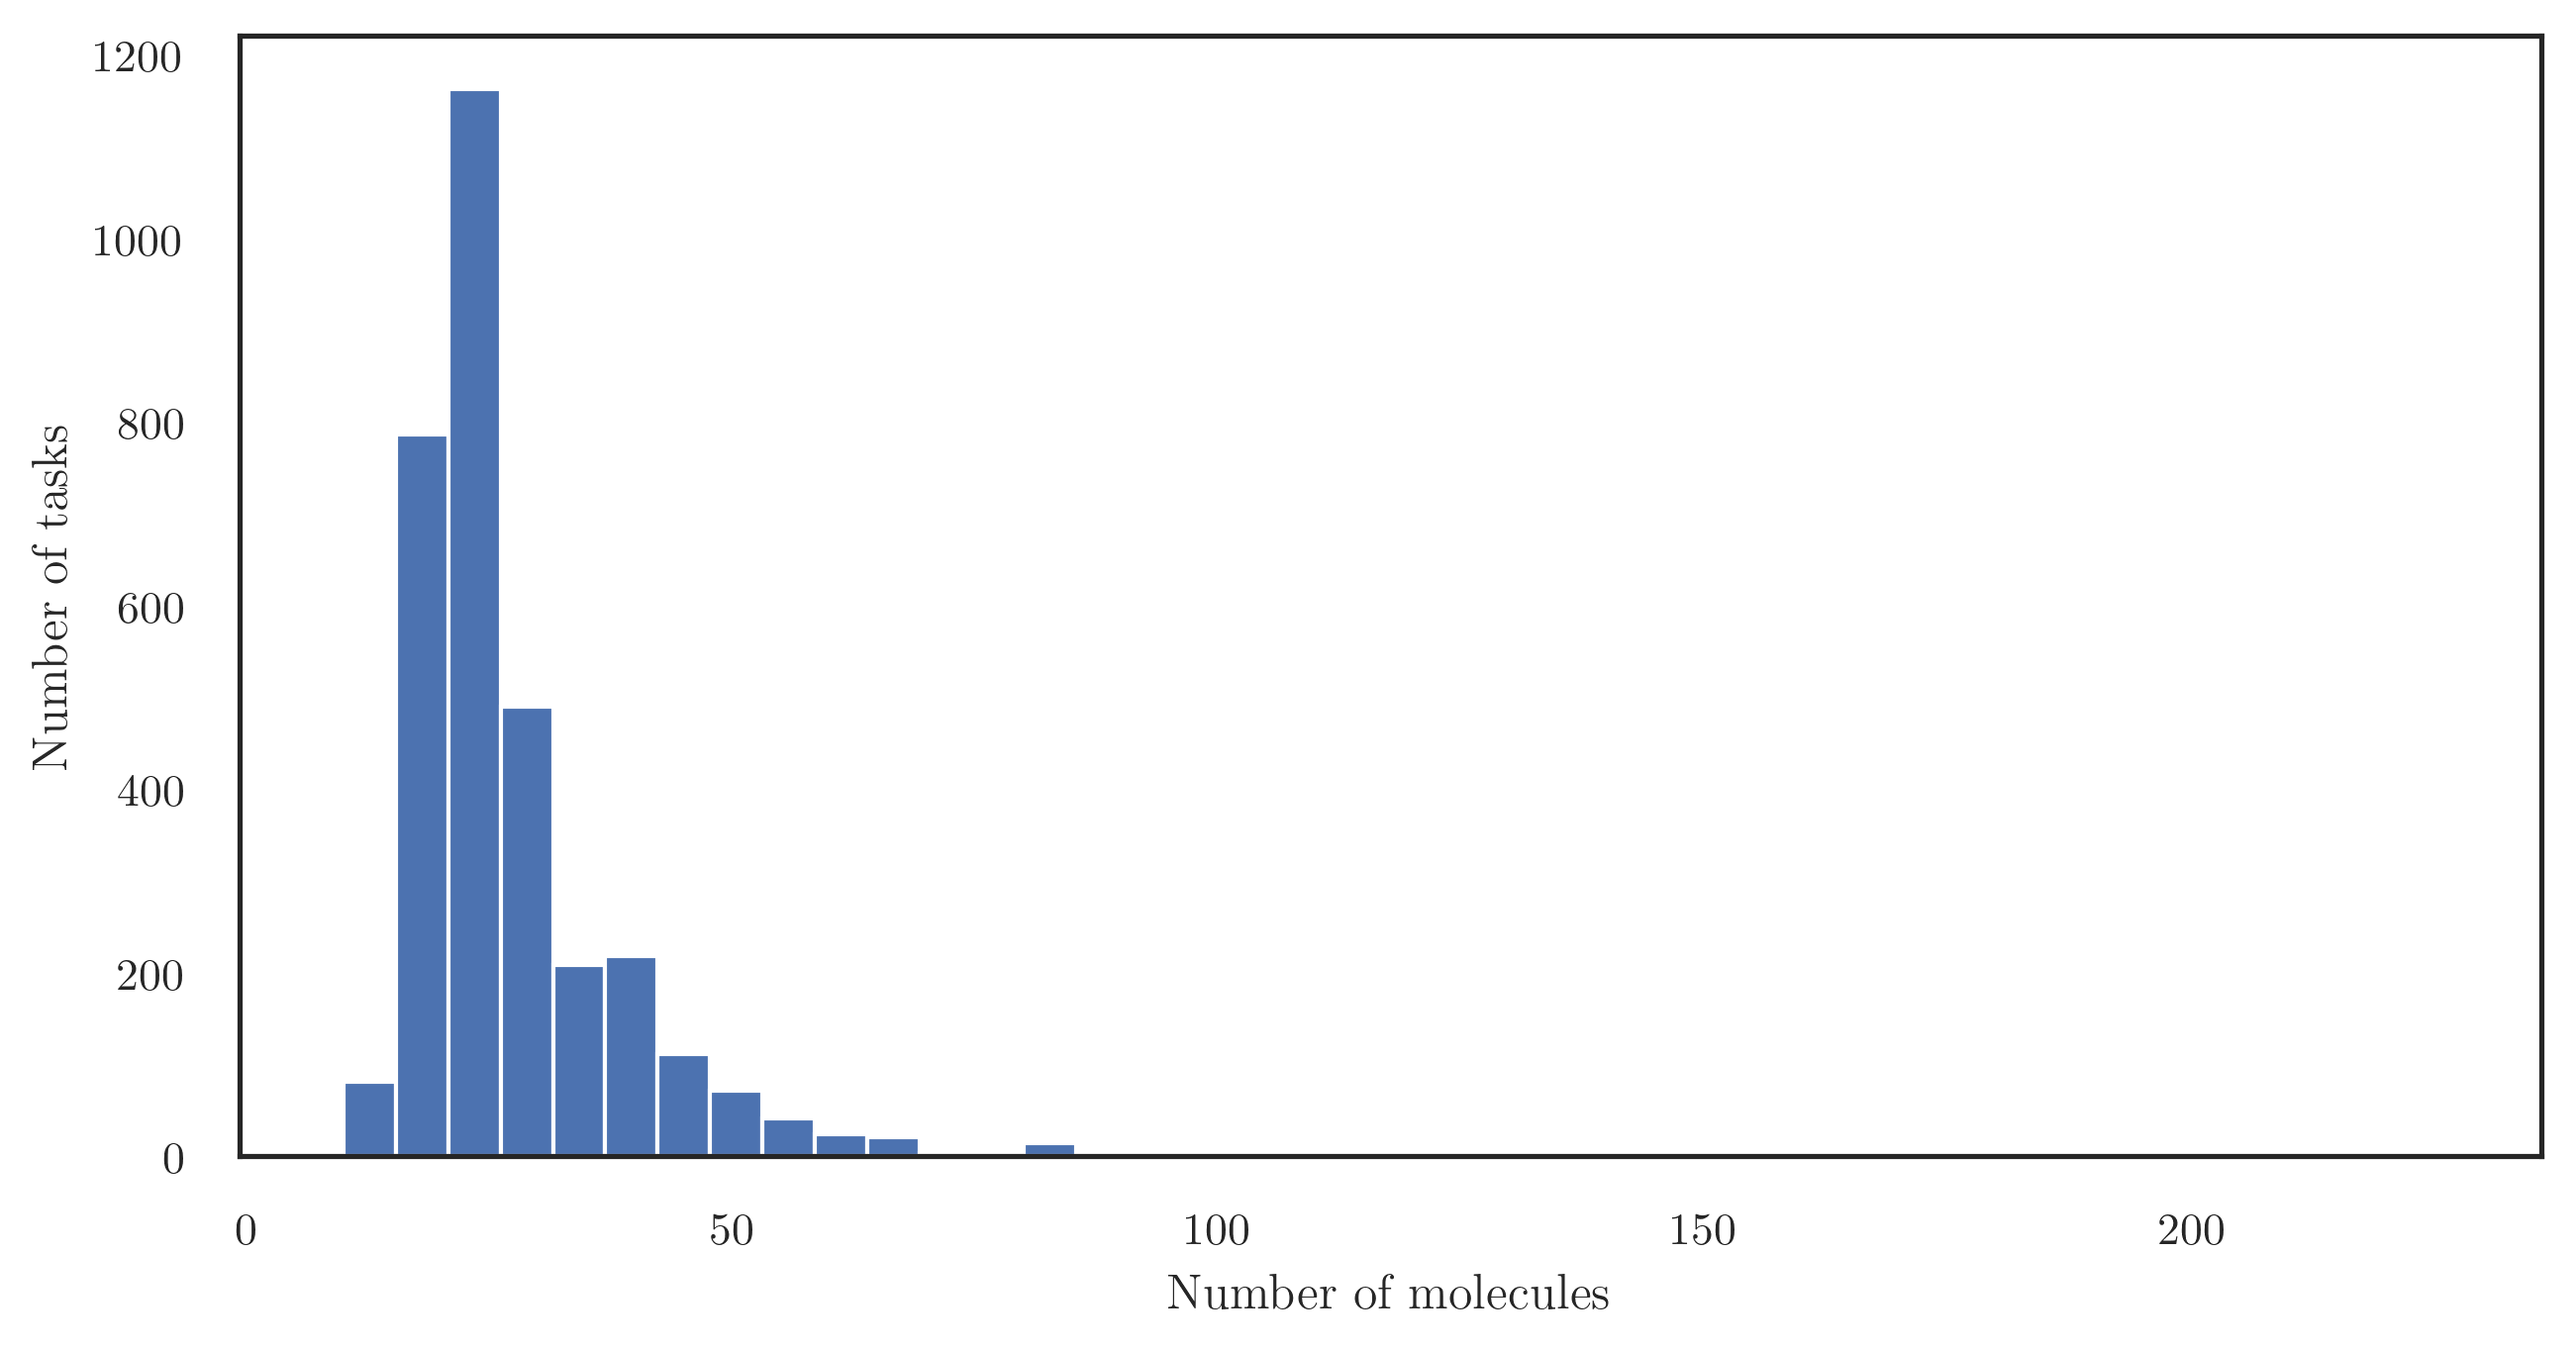
\includegraphics[width=1\textwidth,center]{datasets/hist-antibacterial}
      \caption{\texttt{Antibacterial}}
      \label{fig:hist-antibacterial}
    \end{subfigure}
  }
  \caption{Distribution of the number of examples in each task\\for the \texttt{Binding} and \texttt{Antibacterial} collections}
  \label{fig:histograms}
\end{figure}

\Fig{hist-binding} shows just how scarce data is for both collections, reflecting the time and money needed to perform an exhaustive mapping of the molecular space using \textit{in vitro} and \textit{in vivo} testing.

\subsubsection{\texttt{Binding}}
\label{app:collections-binding}

This collection is extracted from the public database \href{www.bindingdb.org}{BindingDB} \citep{liu2007bindingdb}. We altered it by removing bio-assays with targets correlated above $0.8$ or those with less than 10 experimental measurements, leaving 5,717 tasks.

Each task from the collection reports the binding affinity of small molecules to a target protein. Hence, the task distribution is defined by the characteristics of the proteins.

\subsubsection{\texttt{Antibacterial}}
\label{app:collections-antibacterial}

This task collection is extracted from \href{https://pubchem.ncbi.nlm.nih.gov/}{PubChem} \citep{kim2019pubchem}, a public registery of molecules and bioassays. After also removing bio-assays with correlations above $0.8$ and those with less than 10 samples, we obtain $3,255$ tasks.

Each task in \texttt{Antibacterial} reports the antibacterial effect of a set of small molecules on a given strain of bacterium. More specifically, it describes the minimum concentration needed to wipe out at least half the population of bacteria.

Note that this collection is particularly noisy. Indeed, the results are obtained by testing different concentrations of the same molecules, leading to discrete approximation riddled with thresholding effects.


\subsection{A synthetic collection of molecular data : \texttt{Properties}}
\label{app:collections-properties}

The noise issue in the two bioassay collections led us at InVivo AI to create another meta-dataset, which we called \texttt{Properties}.

Although \texttt{Properties} is a collection of synthetic tasks, it still relates to drug discovery. Hence, is reports a set of 767 computable physico-chemical properties for more than 600,000 molecules, thus completely removing the noise issue while providing a rich benchmarking tool to computational bio-chemists.

With properties, the community can test out algorithms specifically designed for molecular scoring with the challenges it entails (such as the representation issue), while still benefiting from a very large dataset.



\clearpage
\section{Ablation study}
\label{app:ablation}

This section presents more results from the ablation study. See the \href{https://openreview.net/pdf?id=Syeu8CNYvS}{ICLR submission} for a more comprehensive presentation.

\subsection{Task regularisation}
\label{app:ablation-taskreg}

\Tab{app-ablation-tasks} presents the hyper-parameter combinations used in the experiments to assess the impact of the trade-off parameter $\gamma_\mathrm{task}$.
We report the MSE performance obtained on the meta-test for each configuration.

\begin{table}[ht]
  \centering
  \makebox[\linewidth][c]{
  \begin{tabular}{@{}lllllrrr@{}}
    \toprule
                &    &                  &      & $\gamma_\mathrm{task}$ &    0.00 &    0.01 &    0.10 \\
    Conf. & algorithm & K & architecture & $\gamma_\mathrm{pseudo}$ &         &         &         \\
    \midrule
    a & ADKL-KRR & 20 & attention & 0.01 &  0.0585 &  0.0327 &  \textbf{0.0289} \\
    b &             & 10 & deepset & 0.00 &  0.4051 &  \textbf{0.2944} &  0.3671 \\
    c &             &    &                  & 0.10 &  0.4363 &  0.2964 &  \textbf{0.2882} \\
    d & ADKL-GP & 5  & attention & 0.10 &  2.4920 &  \textbf{2.2511} &  2.2994 \\
    e & ADKL-KRR & 20 & attention & 0.00 &  0.0574 &  0.0305 &  \textbf{0.0302} \\
    f & ADKL-GP & 5  & attention & 0.01 &  2.5611 &  \textbf{2.1511} &  2.2112 \\
    g &             &    & deepset & 0.01 &  3.2933 &  \textbf{2.7663} &  3.0971 \\
    h &             & 10 & deepset & 0.01 &  0.7675 &  0.7105 &  \textbf{0.4352} \\
    i &             & 20 & deepset & 0.00 &  0.1201 &  0.0873 &  \textbf{0.0646} \\
    j & ADKL-KRR & 20 & attention & 0.10  & 0.0575 &  0.0447 &  \textbf{0.0273} \\
    \bottomrule
  \end{tabular}}
  \caption{Effect of using task regularisation (parameter $\gamma_\mathrm{task}$) on the MSE performance}
  \label{tab:app-ablation-tasks}
\end{table}

To make reading this table easier, we also repeat \fig{gamma-task} showing the improvement of the MSE relative to $\gamma_\mathrm{task} = 0$ (no regularisation).

\begin{figure}[ht]
  \centering
  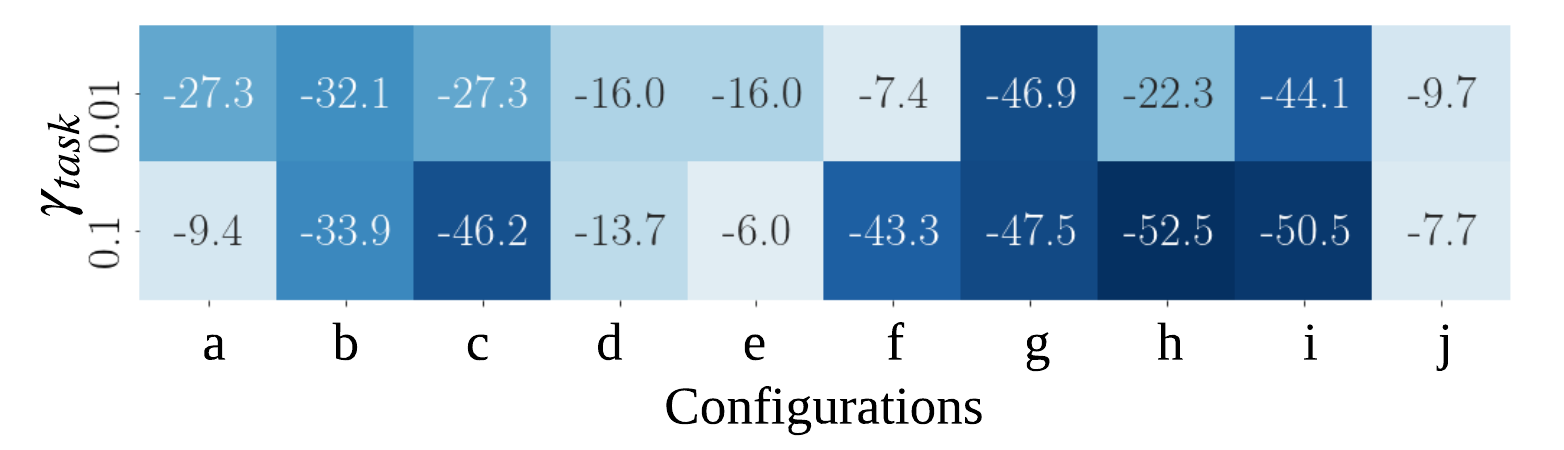
\includegraphics[width=.6\textwidth]{adkl/ablation/gamma-task}
  \caption{Relative improvement of the MSE depending on the $\gamma_\mathrm{task}$ parameter}
  \label{fig:app-mine}
\end{figure}


\subsection{Pseudo representation}
\label{app:ablation-pseudo}

\Tab{app-ablation-pseudo} presents the hyper-parameter combinations used in the experiments to assess the impact of the trade-off parameter $\gamma_\mathrm{pseudo}$, which governs the penalty applied to the divergence between the distribution of learned pseudo-representations and the distribution of actual representations. We also repeat \fig{gamma-pseudo} for better readability.

\begin{table}[ht]
    \caption{Effect of the pseudo-examples regularisation (parameter $\gamma_\mathrm{pseudo}$)\\on the MSE performance}
    \centering
    \begin{tabular}{@{}lllllrrr@{}}
        \toprule
                   &    &                  &      & $\gamma_\mathrm{pseudo}$ &    0.00 &    0.01 &    0.10 \\
        algorithm & K & architecture & $\gamma_\mathrm{task}$ & Conf. &         &         &         \\
        \midrule
        ADKL-GP & 10 & deepset & 0.10 & a  &  0.6079 &  \textbf{0.4352} &  0.5244 \\
                   & 20 & deepset & 0.01 & b  &  0.0873 &  \textbf{0.0761} &  0.0882 \\
        ADKL-KRR & 20 & deepset & 0.00 & c  &  0.0526 &  \textbf{0.0375} &  0.0380 \\
        ADKL-GP & 5  & attention & 0.10 & d  &  2.2801 &  \textbf{2.2112} &  2.2994 \\
        ADKL-KRR & 20 & deepset & 0.01 & e  &  0.0535 &  \textbf{0.0325} &  \textbf{0.0325} \\
        ADKL-GP & 5  & deepset & 0.01 & f  &  2.9466 &  2.7663 &  \textbf{2.7121} \\
                   & 20 & attention & 0.10 & g  &  0.1147 &  0.1144 &  \textbf{0.0870} \\
                   &    & deepset & 0.00 & h  &  0.1201 &  0.0958 &  \textbf{0.0940} \\
                   & 5  & attention & 0.01 & i  &  3.1136 &  \textbf{2.1511} &  2.2511 \\
                   &    &                  & 0.00 & j &  2.8528 &  2.5611 &  \textbf{2.4920} \\
        \bottomrule
    \end{tabular}
    \label{tab:app-ablation-pseudo}
\end{table}

\begin{figure}[ht]
    \centering
    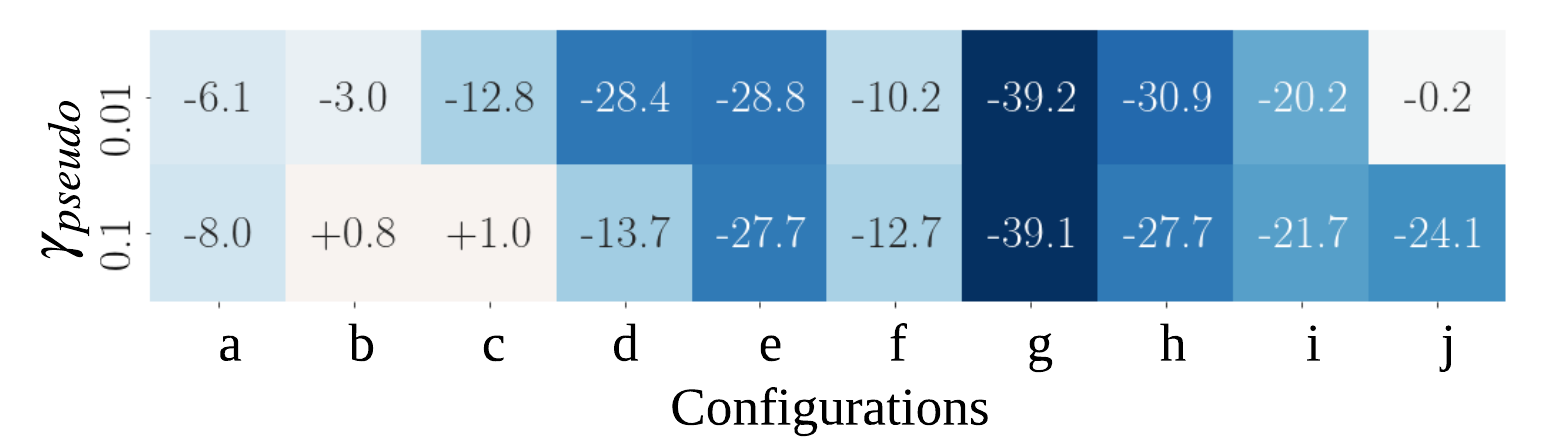
\includegraphics[width=.6\textwidth]{adkl/ablation/heatmap_pseudo}
    \caption{Relative improvement of the MSE depending on the $\gamma_\mathrm{task}$ parameter}
    \label{fig:app-pseudo}
\end{figure}

% Overall, the effect of the regularisation is beneficial, even though we witness a few pathological cases.

\subsection{Joint impact of the task and pseudo-representation regularisations}
\label{app:ablation-task-pseudo}

Since both $\gamma_\mathrm{task}$ and $\gamma_\mathrm{pseudo}$ have a high impact on the training and the generalization performance, we need to assess the relationship between the two.
\Fig{app-pseudo-task} shows for different values of $|\Dsupport|$ the relative improvement of the test MSE compared to the case where no regularisation is done.
Overall, higher is better in both dimensions, although there seems to be a sweet spot on the grid for each value of $|\Dsupport|$ and therefore we can only advise the user to cross-validate on those hyper-parameters.


\begin{figure}[ht]
    \centering
    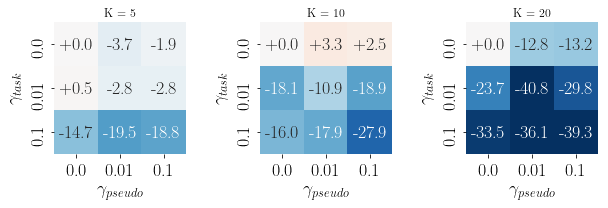
\includegraphics[width=.7\textwidth]{adkl/ablation/heatmap_task_pseudo_metakrr_mk2.png}
    \caption{Average relative improvement of the MSE\\and joint impact of $\gamma_\mathrm{task}$ and $\gamma_\mathrm{pseudo}$.}
    \label{fig:app-pseudo-task}
\end{figure}


\clearpage
\section{Prediction curves on the Sinusoids collection}
\label{app:predictions}

\Fig{app-predictions} presents a visualization of the results obtained by each model on three tasks taken randomly from the meta-test set in the \texttt{Sinusoids} collection.

\begin{figure}[ht]
    \centering
    \begin{subfigure}{.3\textwidth}
        \centering
        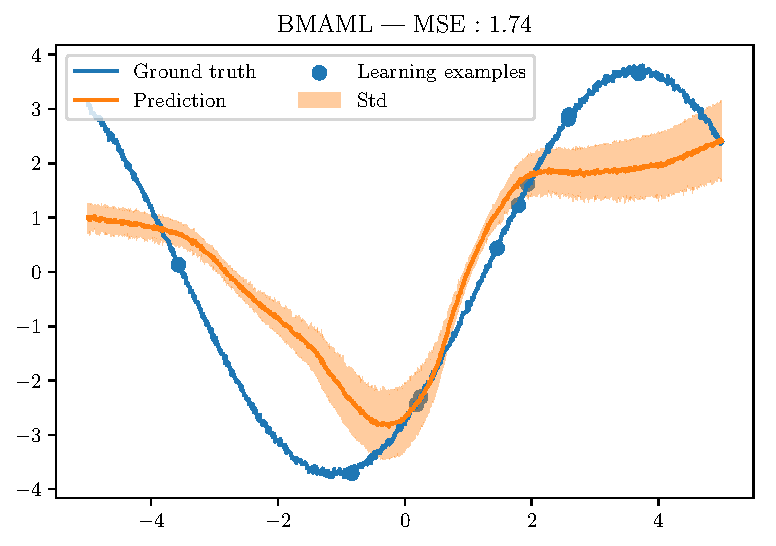
\includegraphics[width=\textwidth]{adkl/predictions/BMAML-18}
    \end{subfigure}
    \hfill
    \begin{subfigure}{.3\textwidth}
        \centering
        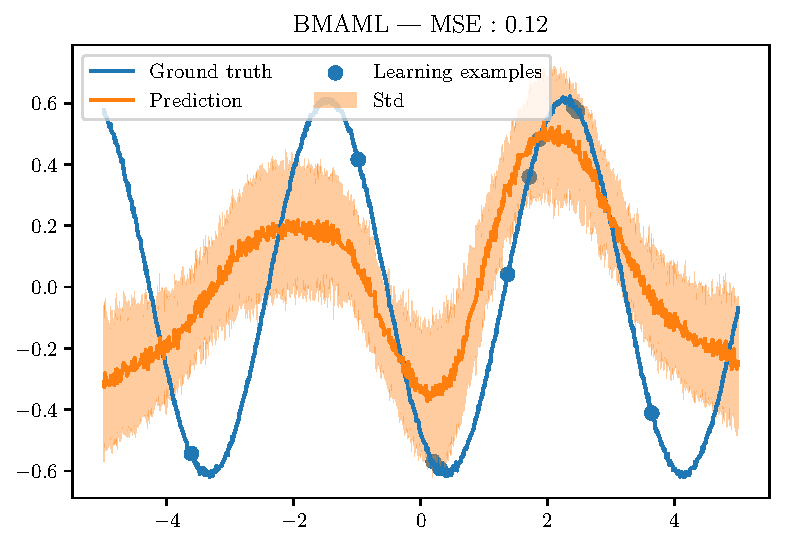
\includegraphics[width=\textwidth]{adkl/predictions/BMAML-15}
    \end{subfigure}
    \hfill
    \begin{subfigure}{.3\textwidth}
        \centering
        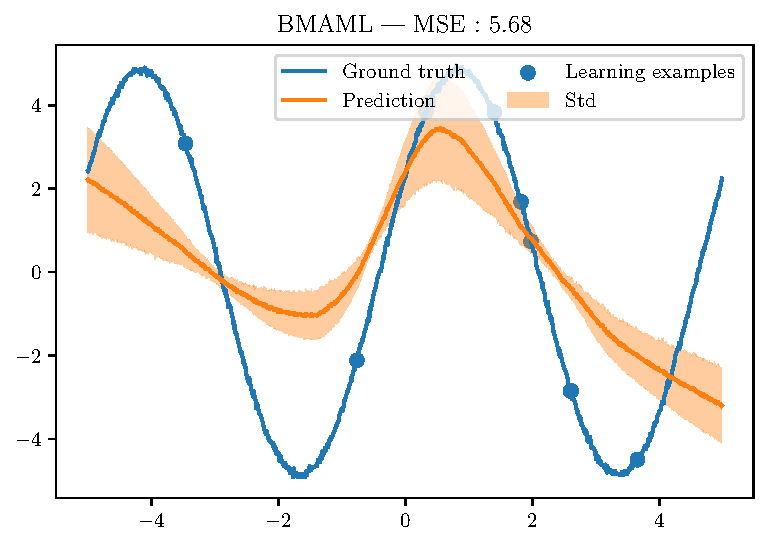
\includegraphics[width=\textwidth]{adkl/predictions/BMAML-4}
    \end{subfigure}
    \\
    \begin{subfigure}{.3\textwidth}
        \centering
        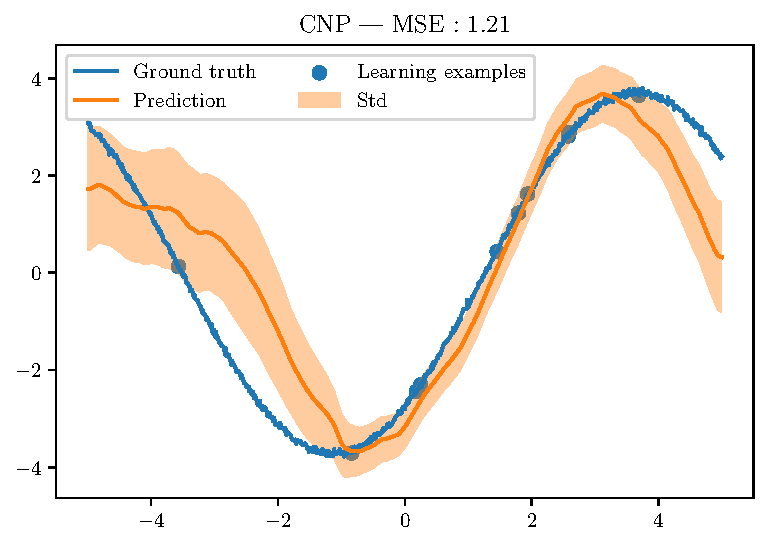
\includegraphics[width=\textwidth]{adkl/predictions/CNP-18}
    \end{subfigure}
    \hfill
    \begin{subfigure}{.3\textwidth}
        \centering
        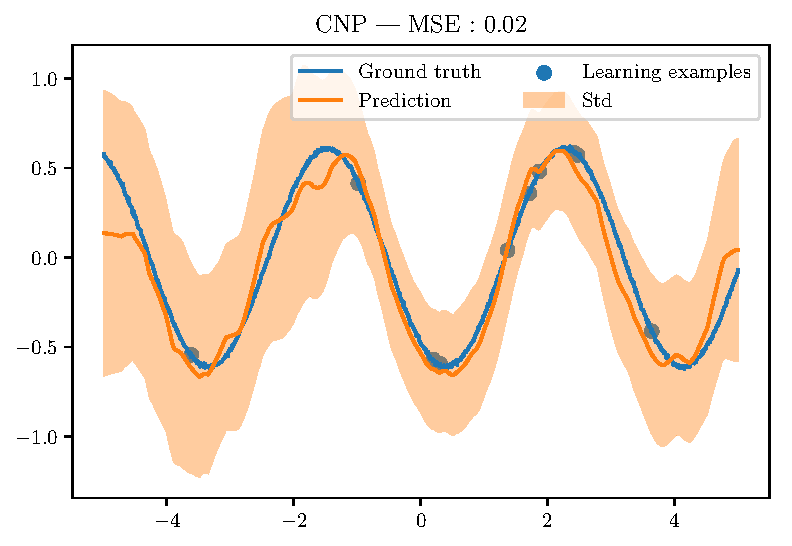
\includegraphics[width=\textwidth]{adkl/predictions/CNP-15}
    \end{subfigure}
    \hfill
    \begin{subfigure}{.3\textwidth}
        \centering
        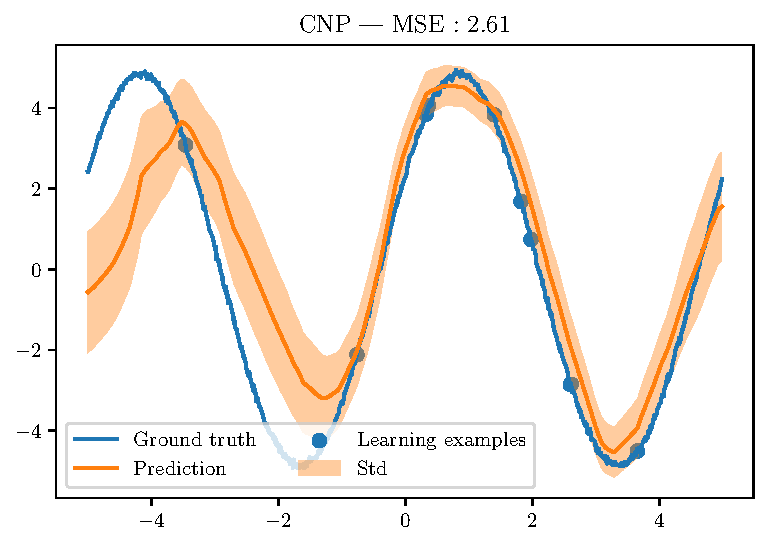
\includegraphics[width=\textwidth]{adkl/predictions/CNP-4}
    \end{subfigure}
    \\
    \begin{subfigure}{.3\textwidth}
        \centering
        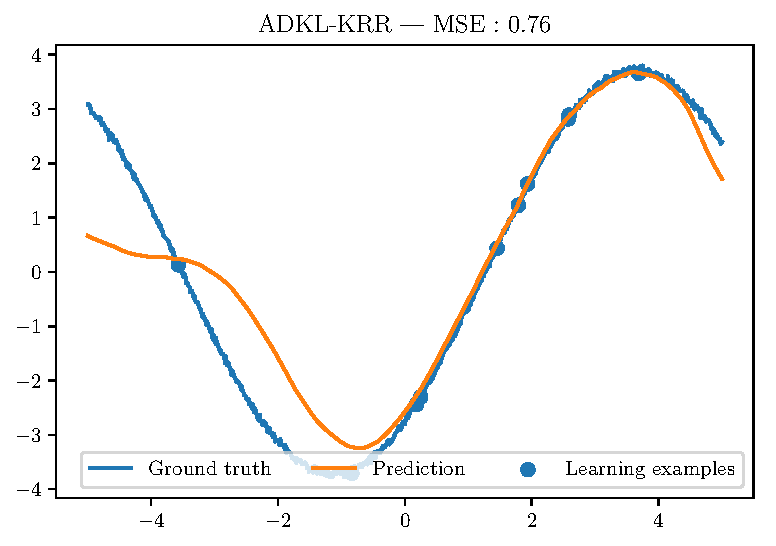
\includegraphics[width=\textwidth]{adkl/predictions/ADKL-KRR-18}
    \end{subfigure}
    \hfill
    \begin{subfigure}{.3\textwidth}
        \centering
        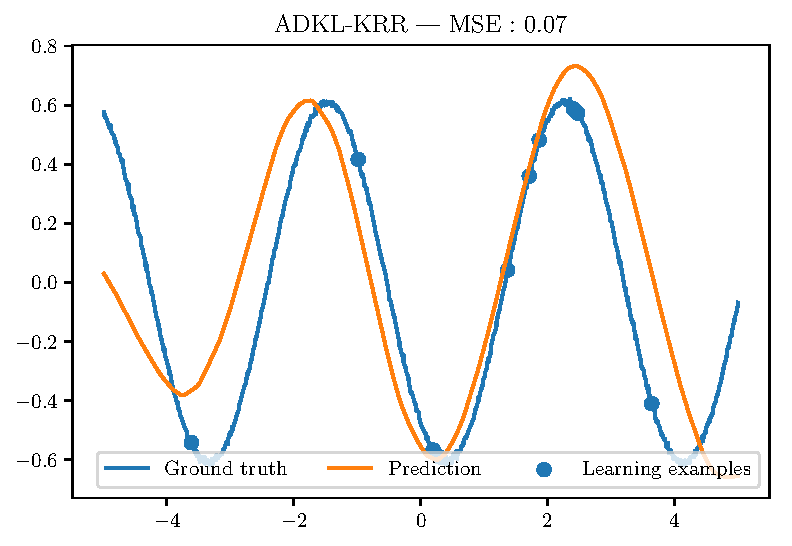
\includegraphics[width=\textwidth]{adkl/predictions/ADKL-KRR-15}
    \end{subfigure}
    \hfill
    \begin{subfigure}{.3\textwidth}
        \centering
        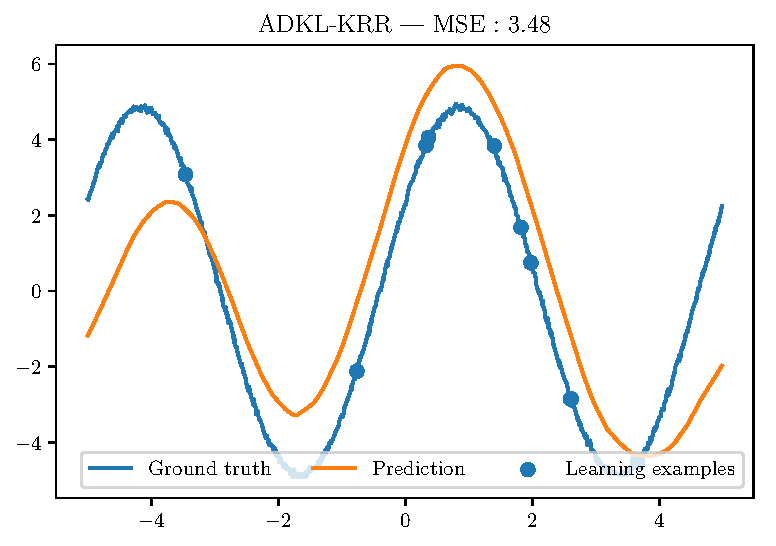
\includegraphics[width=\textwidth]{adkl/predictions/ADKL-KRR-4}
    \end{subfigure}
    \\
    \begin{subfigure}{.3\textwidth}
        \centering
        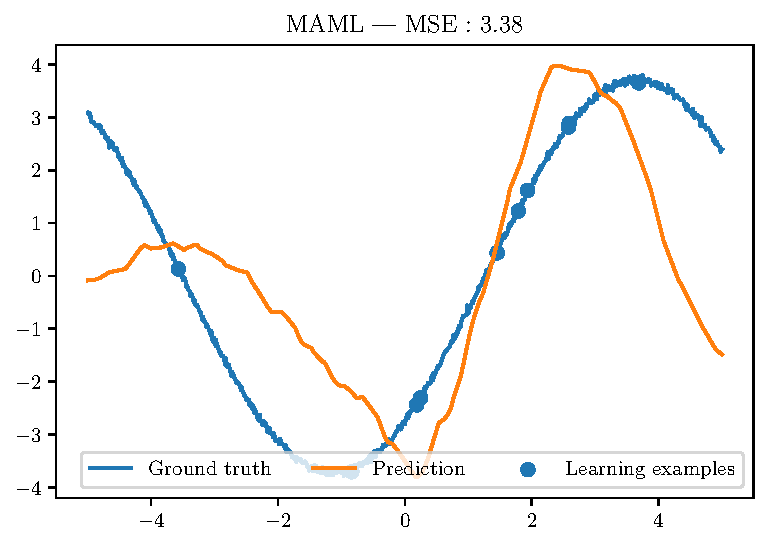
\includegraphics[width=\textwidth]{adkl/predictions/MAML-18}
    \end{subfigure}
    \hfill
    \begin{subfigure}{.3\textwidth}
        \centering
        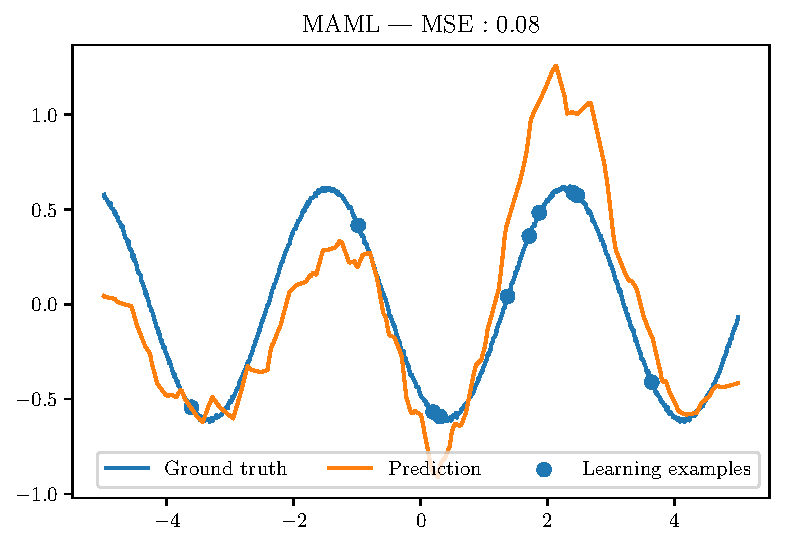
\includegraphics[width=\textwidth]{adkl/predictions/MAML-15}
    \end{subfigure}
    \hfill
    \begin{subfigure}{.3\textwidth}
        \centering
        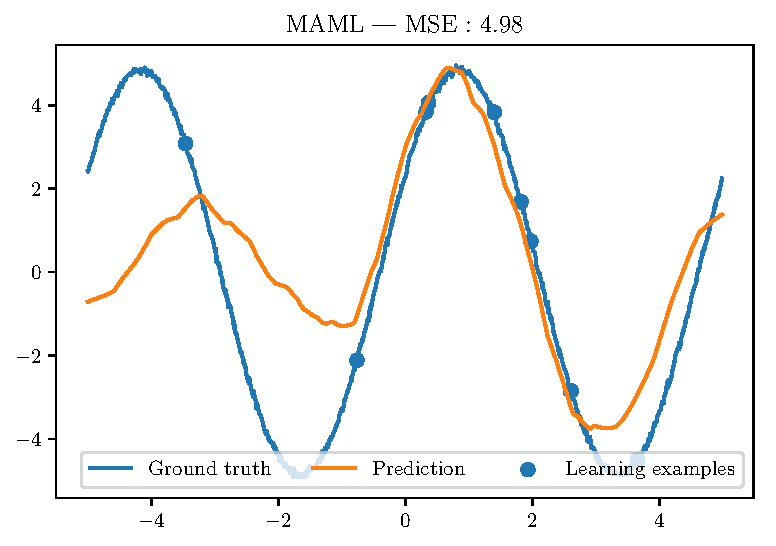
\includegraphics[width=\textwidth]{adkl/predictions/MAML-4}
    \end{subfigure}
    \\
    \begin{subfigure}{.3\textwidth}
        \centering
        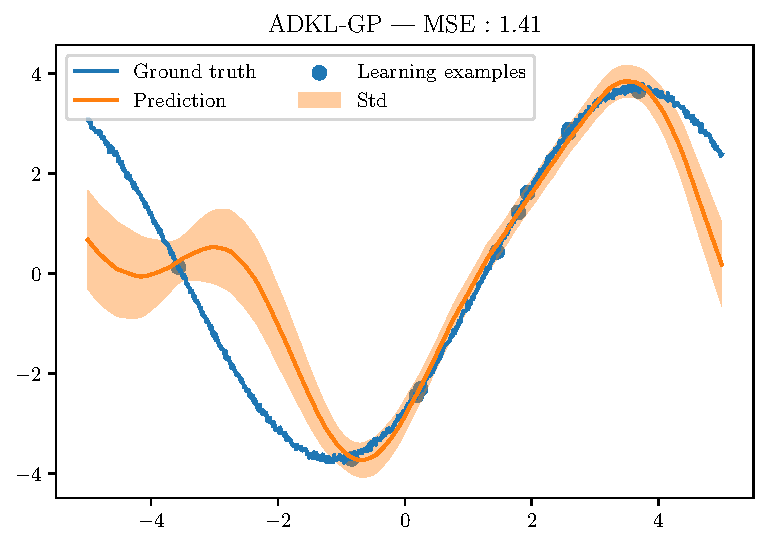
\includegraphics[width=\textwidth]{adkl/predictions/ADKL-GP-18}
    \end{subfigure}
    \hfill
    \begin{subfigure}{.3\textwidth}
        \centering
        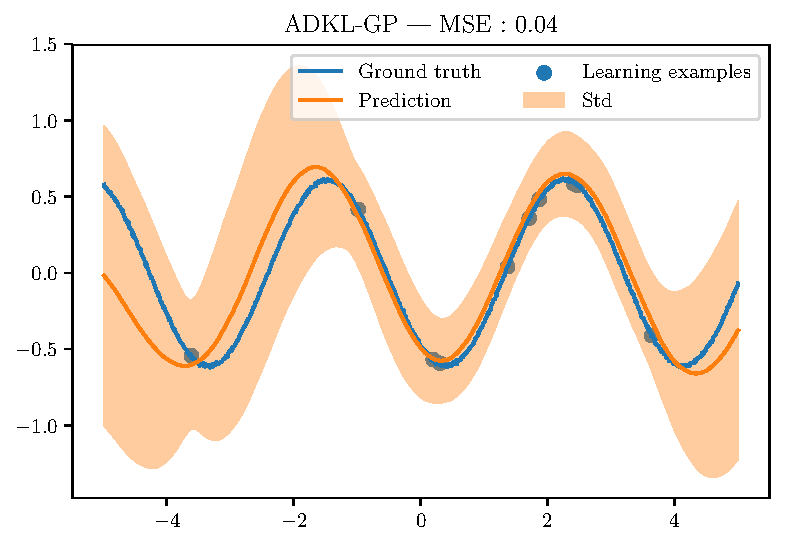
\includegraphics[width=\textwidth]{adkl/predictions/ADKL-GP-15}
    \end{subfigure}
    \hfill
    \begin{subfigure}{.3\textwidth}
        \centering
        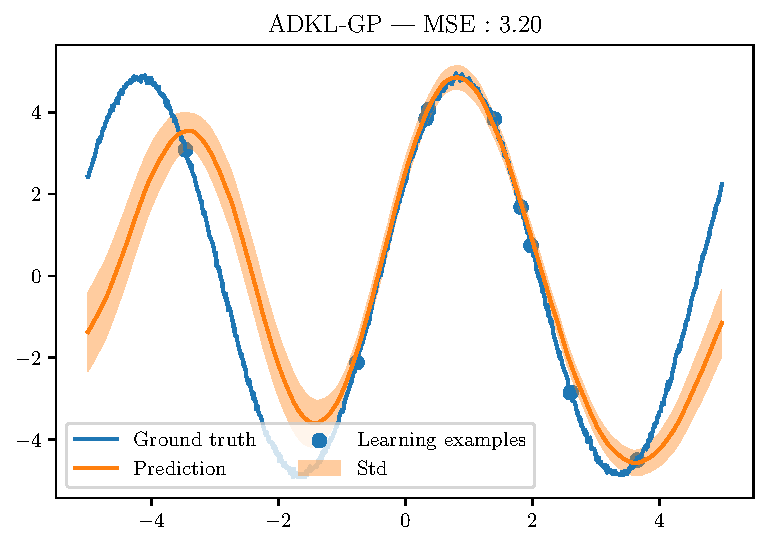
\includegraphics[width=\textwidth]{adkl/predictions/ADKL-GP-4}
    \end{subfigure}
    % \\
    % \begin{subfigure}{.3\textwidth}
    %     \centering
    %     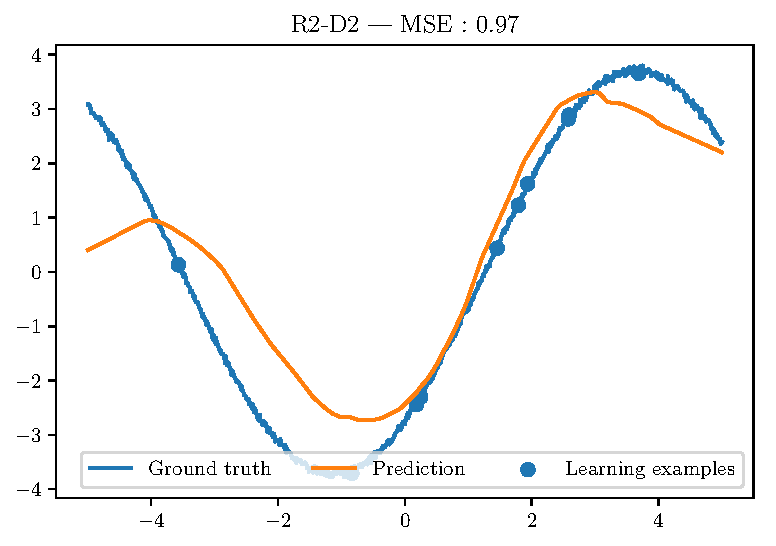
\includegraphics[width=\textwidth]{adkl/predictions/R2-D2-18}
    % \end{subfigure}
    % \hfill
    % \begin{subfigure}{.3\textwidth}
    %     \centering
    %     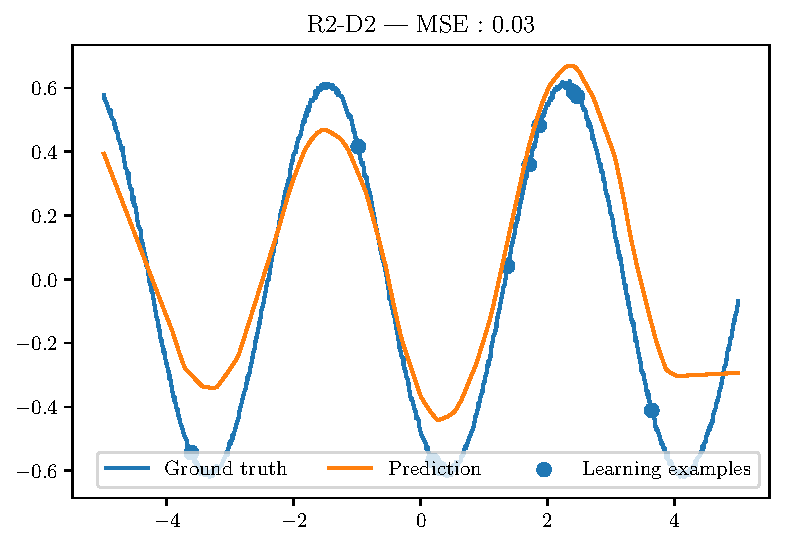
\includegraphics[width=\textwidth]{adkl/predictions/R2-D2-15}
    % \end{subfigure}
    % \hfill
    % \begin{subfigure}{.3\textwidth}
    %     \centering
    %     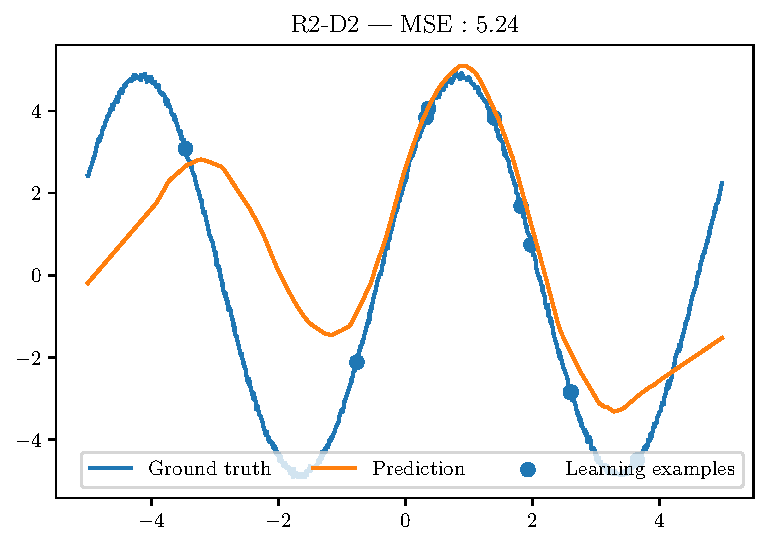
\includegraphics[width=\textwidth]{adkl/predictions/R2-D2-4}
    % \end{subfigure}
    \caption{Meta-test time predictions on the \texttt{Sinusoids} collection}
    \label{fig:app-predictions}
\end{figure}
